%% LyX 2.3.6 created this file.  For more info, see http://www.lyx.org/.
%% Do not edit unless you really know what you are doing.
\documentclass[english,aspectratio=169]{beamer}
\usepackage{lmodern}
\renewcommand{\sfdefault}{lmss}
\renewcommand{\ttdefault}{lmtt}
\usepackage[T1]{fontenc}
\usepackage[latin9]{inputenc}
\setlength{\parskip}{\medskipamount}
\setlength{\parindent}{0pt}
\usepackage{amssymb}
\usepackage{graphicx}

\makeatletter

%%%%%%%%%%%%%%%%%%%%%%%%%%%%%% LyX specific LaTeX commands.
\pdfpageheight\paperheight
\pdfpagewidth\paperwidth


%%%%%%%%%%%%%%%%%%%%%%%%%%%%%% Textclass specific LaTeX commands.
% this default might be overridden by plain title style
\newcommand\makebeamertitle{\frame{\maketitle}}%
% (ERT) argument for the TOC
\AtBeginDocument{%
  \let\origtableofcontents=\tableofcontents
  \def\tableofcontents{\@ifnextchar[{\origtableofcontents}{\gobbletableofcontents}}
  \def\gobbletableofcontents#1{\origtableofcontents}
}

%%%%%%%%%%%%%%%%%%%%%%%%%%%%%% User specified LaTeX commands.
\usetheme{AnnArbor}
\usecolortheme{seagull}
\hypersetup{}
\usepackage{tikz}
\usepackage{color}
\usepackage{listings}

\makeatother

\usepackage{babel}
\begin{document}
\title[M7-2]{Friction and Turbulence}
\author{Department of Oceanography}
\institute[UCT]{University of Cape Town}
\date{SEA3004F}
\makebeamertitle

\section*{Outlines}
\begin{frame}{Outline}

\tableofcontents{}
\end{frame}


\section{Oceanic scales and marine ecosystems}
\begin{frame}{Scales in the physical ocean}

\begin{columns}[t]

\column{7.5cm}

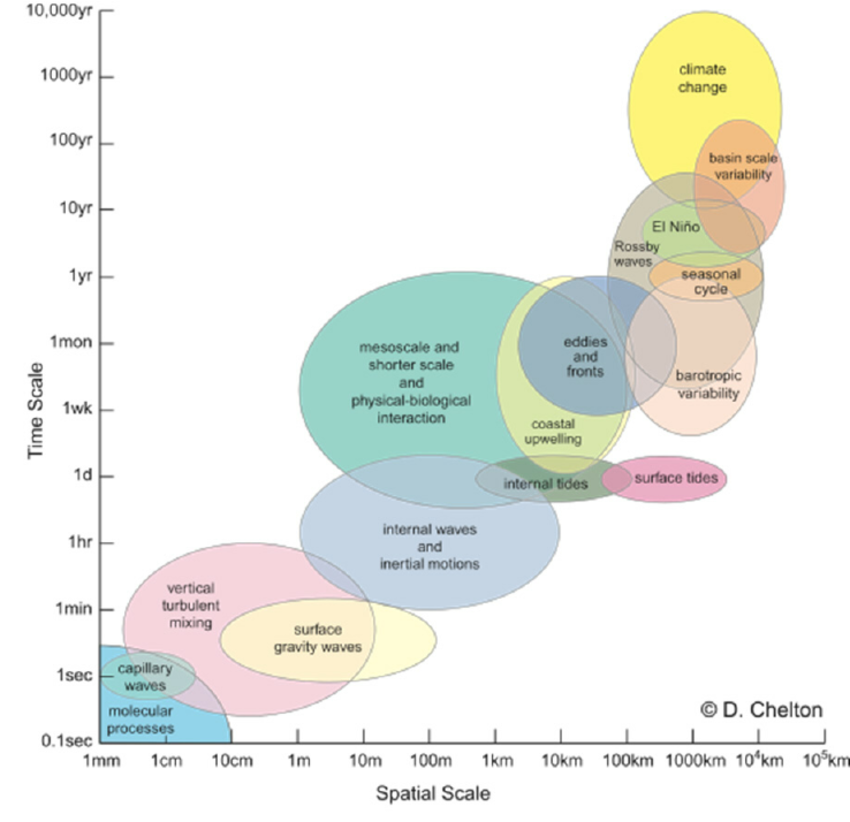
\includegraphics[width=6.5cm]{../figures/M7/Time-and-space-scales-of-ocean-variability-courtesy-D-Chelton-Oregon-State-University}

{\scriptsize{}Main time and space scales of ocean variability (D.
Chelton, Oregon State University, after Dickey (2001)). }{\scriptsize\par}

\column{7cm}

{\scriptsize{}We generally observe some relationships between the
spatial and the temporal scales (large phenomena occurs at longer
time scales, such as El Nino), although certain processes overlap
and span several orders of magnitude (note that the scales of the
axes are not linear).}{\scriptsize\par}

{\scriptsize{}This figure is often associated to the concept of the
}\textbf{\scriptsize{}energy cascade}{\scriptsize{}: the energy cascades
from the larger scales into the smaller scales and dissipates. This
should not be interpreted literally: it does not mean that a system
that is highly variable at the smaller scales will be highly variable
at the larger scales. }{\scriptsize\par}

{\scriptsize{}It means that the energy at the larger scale is transferred
through various processes to the smaller scales, but the resulting
variability (i.e. the way the system fluctuates around a long term
mean) can be a complex combination of several scales. }{\scriptsize\par}
\end{columns}

\end{frame}

\begin{frame}{Physical-biological interactions in marine ecosystems}

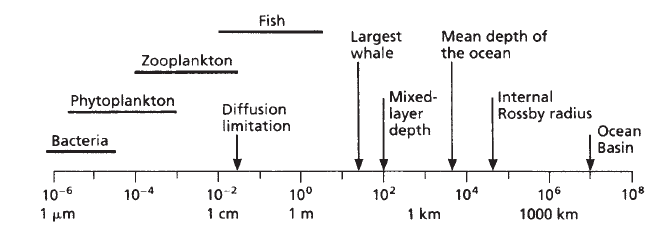
\includegraphics[width=10cm]{../figures/M7/scales_mann_lazier}
\begin{itemize}
\item {\scriptsize{}It is useful to have a feeling for the dimensions of
the organisms and phenomena to be discussed (Fig. 1.01, Mann and Lazier,
2006). Ocean basins are typically 10,000 km wide and confine the largest
biological communities. Mesoscale processes (i.e. in the order of
100 km in space and in the order of weeks in time) are the main source
of variability in water masses and affect the distribution of nutrients
and organisms. The average depth of the ocean is 3800 m but the depths
of the euphotic layer (\textasciitilde 100 m) and the mixed layer
(\textasciitilde 100 m) are more often critical to open-ocean biological
processes. }{\scriptsize\par}
\item {\scriptsize{}All marine organisms live at scales that are much smaller
than the mesoscale or sub-mesoscale processes, and the ocean mixed
layer. The base of the food web in the ocean, the plankton ecosystem,
is therefore largely affected by processes at the microscale.}{\scriptsize\par}
\end{itemize}
\end{frame}


\section{The concept of friction}
\begin{frame}{Frictional processes}

\begin{columns}[t]


\column{7.5cm}
\begin{itemize}
\item {\footnotesize{}This picture was taken under a strong gale of 26 m
s$^{-1}$ in the Bay of Biscay (France) looking upwind, but is common
everywhere in the Southern Ocean. Breaking is occurring at the crests
of the larger waves, separated by over 100 m, and there are numerous
bands of foam aligned in the downwind direction, as well as evidence
of short waves with a typical wavelength of about 20 cm (image taken
from: An Introduction to Ocean Turbulence by S. A. Thorpe)}{\footnotesize\par}
\item {\footnotesize{}Energy from the wind is transferred to the ocean by
means of turbulent processes. Most of the visible effects of the ocean
are driven by frictional processes. }{\footnotesize\par}
\end{itemize}

\column{6cm}

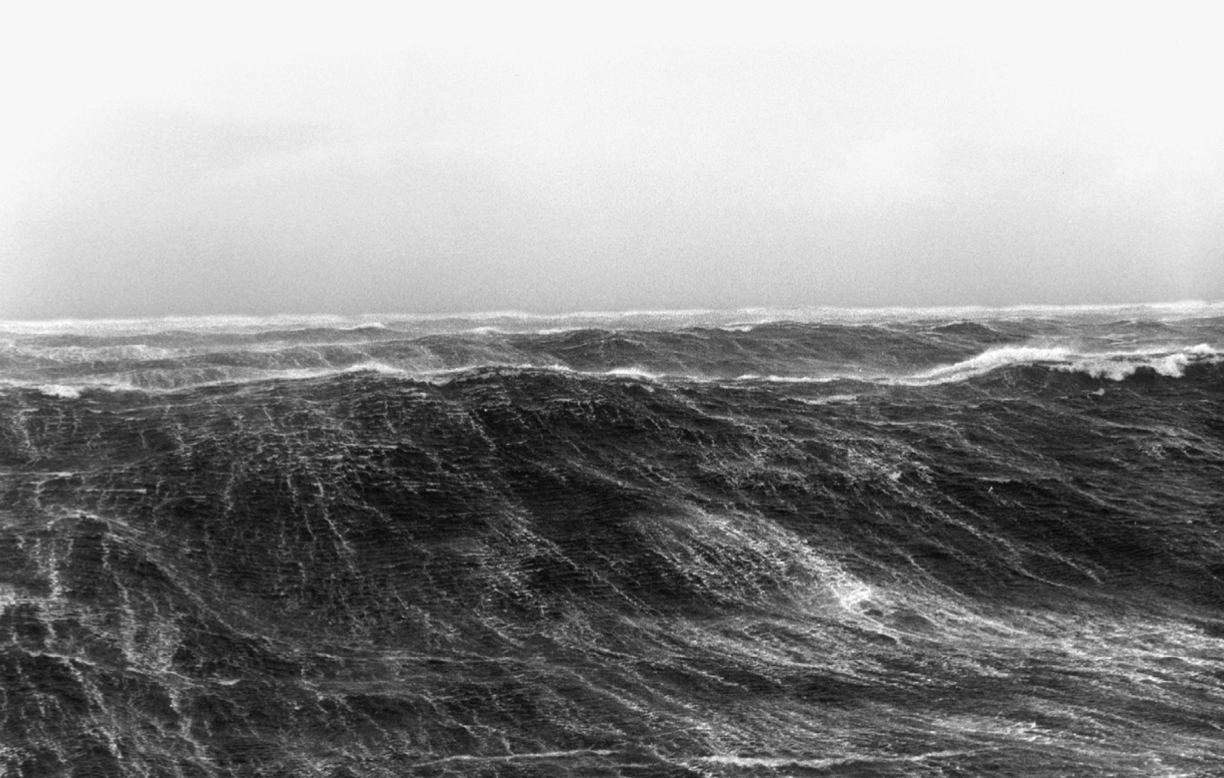
\includegraphics[width=6cm]{../figures/M7/ocean_turbulence_waves}
\begin{itemize}
\item {\footnotesize{}How does the momentum propagates from the molecular
scales to the scales of the waves and to the general circulation of
the ocean?}{\footnotesize\par}
\end{itemize}
\end{columns}

\end{frame}

\begin{frame}{Friction and viscosity }

\begin{columns}

\column{5cm}

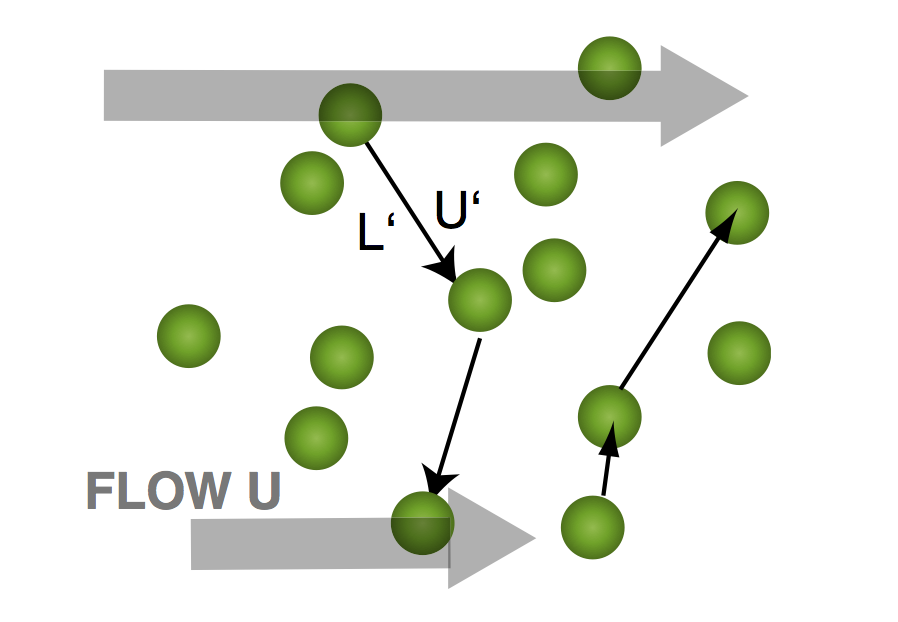
\includegraphics[width=6cm]{../figures/M7/viscosity}

\column{6cm}

\textbf{\footnotesize{}Friction}{\footnotesize{} is usually described
as the resistance to motion. Friction between two solid bodies dissipates
motion (the kinetic energy) into heat and slows down the relative
movement.}\textbf{\footnotesize{} In a fluid, friction leads to the
transfer of momentum between different parts of the fluid itself.}{\footnotesize{}
The physical process that }\emph{\footnotesize{}transmits momentum}{\footnotesize{}
is called }\textbf{\footnotesize{}viscosity}{\footnotesize{}, which
is an inherent property of the fluid.}{\footnotesize\par}
\end{columns}

{\footnotesize{}In a very simplified view, a fluid can be thought
of being composed of different layers, each one with several molecules,
as in the figure above. If the layers slide on each other, the motion
is called }\emph{\footnotesize{}laminar flow}{\footnotesize{}. Momentum
exchange in a laminar flow occurs as a result of the transfer of molecules
with different velocities between adjacent layers: }\textbf{\footnotesize{}this
process is called molecular viscosity}{\footnotesize{}. Molecular
viscosity is found to be proportional to the mean velocity of the
molecules $\left|U'\right|$ and the mean pathway $\left|L'\right|$.
Units are m$^{2}$s$^{-1}$}{\footnotesize\par}
\end{frame}

\begin{frame}{Dynamic viscosity, kinematic viscosity and momentum flux }

\begin{itemize}
\item {\small{}The molecular viscosity is expressed by means of two quantities:
}\textbf{\small{}dynamic viscosity and kinematic viscosity}{\small{}.
Dynamic viscosity ultimately depends on the fluid density, while kinematic
viscosity depends on the inherent fluid features. If a fluid responds
to a surface stress by generating a proportional change in the velocity
measured in the interior, it is called a }\textbf{\small{}Newtonian
fluid}{\small{}. }{\small\par}
\item {\small{}We recall that stress is a force per unit area, with the
units of pressure. In a Newtonian fluid, viscous stresses are linearly
proportional to the spatial variations of velocity
\[
\vec{\tau_{u}}\propto\left(\frac{\partial u}{\partial x},\frac{\partial u}{\partial y},\frac{\partial u}{\partial z}\right)
\]
The RHS is called the velocity shear or the fluid strain. The proportionality
constant is called }\textbf{\small{}dynamic viscosity}{\small{} $\mu$,
which has units of kg m$^{-1}$ s$^{-1}$.}\textbf{\small{} NB:}{\small{}
}\emph{\small{}the formula shows the stress and shear relation in
the x-direction}{\small{}. The stress is actually a tensor, that is
a matrix. }{\small\par}
\item {\small{}Dynamic viscosity is the product between density and kinematic
viscosity, $\mu=\rho\nu$. In practice, we usually work with the }\textbf{\small{}kinematic
viscosity}{\small{} $\nu$, which has units of m$^{2}$ s$^{-1}$.
Kinematic viscosity is }\emph{\small{}isotropic}{\small{} and depends
on temperature ($10^{-6}$ m$^{2}$ s$^{-1}$ at 20$^{\circ}C$).}{\small\par}
\end{itemize}
\end{frame}

\begin{frame}{Momentum flux due to friction}

\begin{center}
\vspace{-0.5cm}
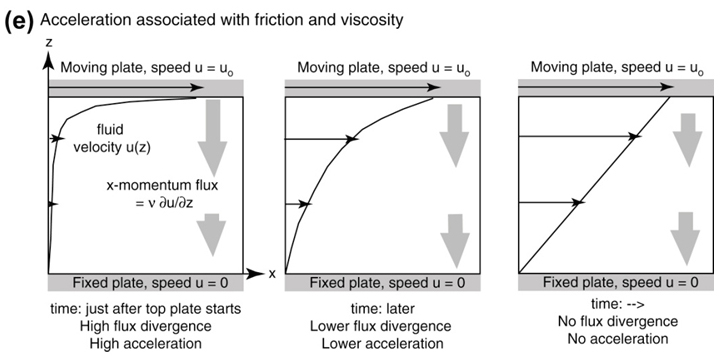
\includegraphics[scale=0.6]{../figures/M7/viscous_forces_talley}
\par\end{center}
\begin{itemize}
\item \vspace{-0.5cm}
{\scriptsize{}The acceleration of the flow depends on changes in the
viscous stress from one point to another). The figure above (Talley,
Ch S7) illustrates the momentum transfer from a plate that is set
into motion at the surface of the fluid until the equilibrium flow
is reached. When the velocity changes linearly from top to bottom
as in the final stage above, this condition is called Couette flow. }{\scriptsize\par}
\item {\scriptsize{}Momentum flux has units of m$^{2}$ s$^{-2}$ (it is
actually a velocity being transported by the velocity field!). The
acceleration resulting from the momentum flux which goes in the momentum
equations is obtained from the divergence of the viscous stress along
x, which given the constant and isotropic nature of kinematic viscosity
is written as 
\begin{equation}
F_{x}=\nu\nabla\cdot\vec{\tau_{u}}=\nu\left(\frac{\partial}{\partial x}\frac{\partial u}{\partial x}+\frac{\partial}{\partial y}\frac{\partial u}{\partial y}+\frac{\partial}{\partial z}\frac{\partial u}{\partial z}\right)=\nu\left(\frac{\partial^{2}u}{\partial x^{2}}+\frac{\partial^{2}u}{\partial y^{2}}+\frac{\partial^{2}u}{\partial z^{2}}\right)\label{eq:viscous-force}
\end{equation}
}{\scriptsize\par}
\end{itemize}
\end{frame}

\begin{frame}{Heat and salt fluxes: molecular diffusion}

\begin{columns}[t]


\column{7.5cm}
\begin{itemize}
\item {\scriptsize{}The same concept can be extended to the dissipation
of dissolved substances in the water (salt and nutrients) and to the
diffusion of heat through the ocean. (Talley, Chap S7: 7.3). This
process pertains to any diffusion of substances. As the molecules
are moved around randomly, with their own speed, they transport properties. }{\scriptsize\par}
\item \textbf{\scriptsize{}Molecular diffusion is the slow mixing caused
by the random motion of molecules.}{\scriptsize{} Temperature, salt
or nutrients are diffused according to their molecular diffusion rates,
which is larger for heat and smaller for dissolved substances (see
Table in Talley's Chapter S7). }{\scriptsize\par}
\item {\scriptsize{}Small organisms must rely on this flux for their survival.
A very famous paper by the Nobel Prize EM Purcell explains how is
Life at small Reynolds numbers. It is an interesting reading to realize
the complex life of microscopic organisms in the ocean.}{\scriptsize\par}
\end{itemize}

\column{6cm}
\begin{fact}
{\tiny{}The flux of some constituent through the water due to molecular
diffusion is given by }\textbf{\tiny{}Fick\textquoteright s first
law of diffusion}{\tiny{}. This law states that if the concentration
of some constituent C changes by an amount dC over a short distance
dz, the flow of C down the concentration gradient by molecular motion
is
\[
F=-D\frac{dC}{dz}
\]
If $C$ is in kg m$^{-3}$, $F$ is the flux of $C$ in kg m$^{-2}$
s$^{-1}$ then $D$ is the }\textbf{\tiny{}coefficient of molecular
diffusion}{\tiny{} in m$^{2}$ s$^{-1}$ (for large chemical species
such as chloride ion or nitrate is about 1.5 10$^{-9}$ m$^{2}$ s$^{-1}$).
The coefficient $D$ contains information related to how fast the
molecules of the diffusing substance move through the fluid. To use
this information, the definition of D is converted into the formula
$D=l^{2}/t$ to calculate the time it takes for a molecule to go a
distance $l$. Try to estimate the time it would take for a molecule
of nutrient to travel 0.1 mm. (from Mann and Lazier, Dynamics of marine
ecosystems).}{\tiny\par}
\end{fact}

\end{columns}

\end{frame}

\begin{frame}{Viscosity vs molecular diffusion}

\begin{center}
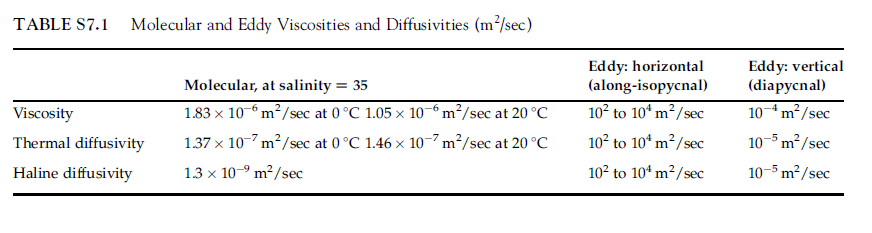
\includegraphics[scale=0.6]{../figures/M7/viscosity_table}
\par\end{center}
\begin{itemize}
\item {\scriptsize{}Table S1 in Talley, Descriptive Physical Oceanography
(Chapter S7) }{\scriptsize\par}
\end{itemize}
\end{frame}


\section{Turbulence in the ocean}
\begin{frame}{Examples of turbulence in the ocean}

The next two slides illustrates two examples of turbulence in the
ocean. The effects of turbulence are usually observed in the uneven
and chaotic distribution of fluid properties, such as temperature. 
\begin{itemize}
\item The first slide shows the vertical mixing induced by the passage of
a hurricane along the US coast. The satellite image demonstrates how
surface temperature was affected by the entrainment of colder water
from the deep. The left panels are the results of an ocean simulation
showing the vertical distribution of temperature before and after
the passage (indicated by the vertical dashed lines). The energy injected
by the strong winds enhance the ocean turbulence, mixing the warmer
surface waters with the waters below the thermocline. The increased
turbulence is visible by the larger values of the eddy viscosity. 
\item The second slide shows the simulation of horizontal eddies in correspondence
with fronts: the equatorial upwelling and the Agulhas-Benguela system.
The scale of turbulence is much larger in horizontal processes.
\end{itemize}
\end{frame}

\begin{frame}{Turbulence in the vertical: response to hurricanes}

\begin{center}
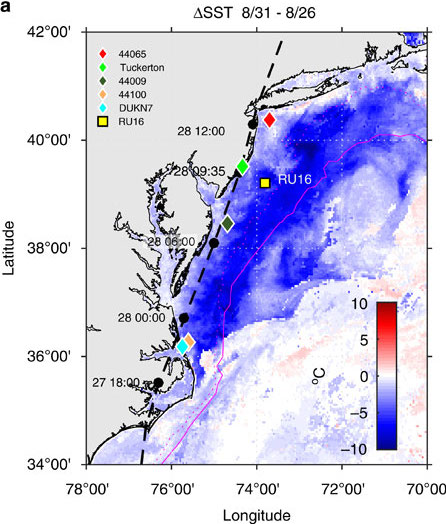
\includegraphics[scale=0.4]{../figures/M7/Irene_DSST_glenn}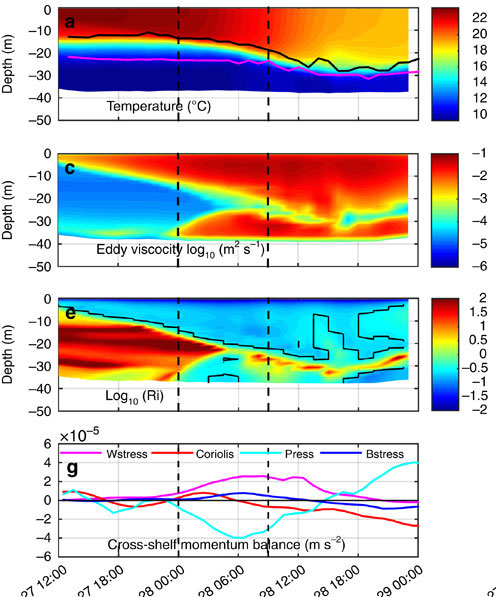
\includegraphics[scale=0.2]{../figures/M7/Irene_glenn_ROMS}
\par\end{center}

\begin{center}
{\tiny{}Glenn et al (2016) Stratified coastal ocean interactions with
tropical cyclones Nature Communications 7 doi:10.1038/ncomms10887}{\tiny\par}
\par\end{center}

\end{frame}

\begin{frame}{Horizontal turbulence: mesoscale}

\begin{center}
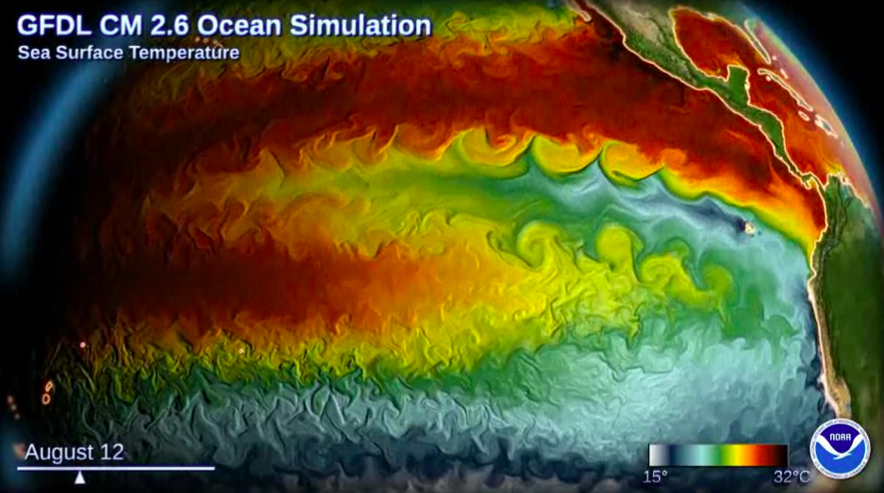
\includegraphics[scale=0.2]{../figures/M7/GFDL_mesoscale}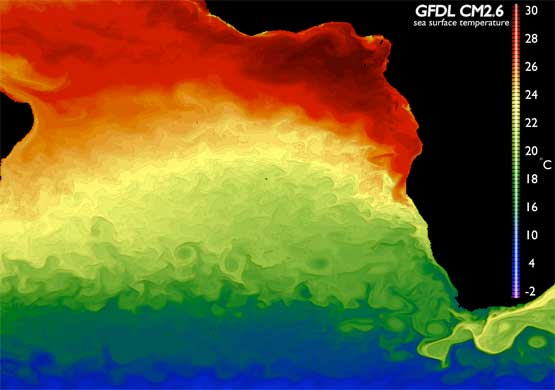
\includegraphics[scale=0.3]{../figures/M7/GFDL_mesoscale_SA}
\par\end{center}

\end{frame}

\begin{frame}{Turbulence}

\begin{center}
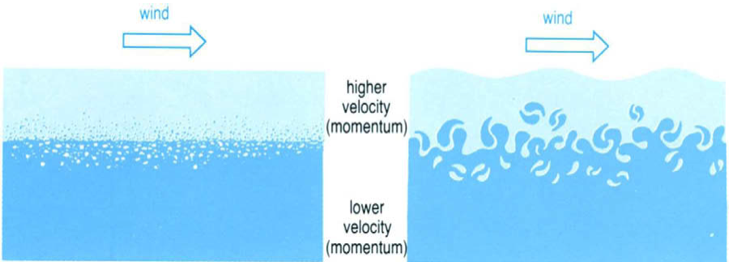
\includegraphics[scale=0.3]{../figures/M7/friction_viscosity}
\par\end{center}
\begin{itemize}
\item {\scriptsize{}At the sea-surface, as in the rest of the ocean, motion
is rarely laminar, but instead }\textbf{\scriptsize{}turbulent}{\scriptsize{},
so that parcels of water, rather than single molecules, are exchanged
between one part of the moving fluid and another. }{\scriptsize\par}
\item {\scriptsize{}This process is described by using the concept of }\textbf{\scriptsize{}eddy
viscosity}{\scriptsize{}, as described at the end of the 19th century
by Osborne Reynolds.}{\scriptsize\par}
\end{itemize}
\end{frame}

\begin{frame}{The Reynolds experiment}

\begin{columns}

\column{5cm }

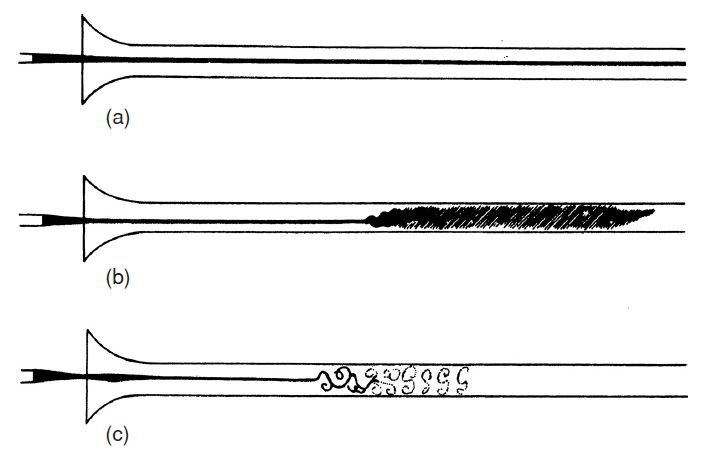
\includegraphics[scale=0.35]{../figures/M7/reynolds_experiment}

\column{6cm }

{\scriptsize{}The }\textbf{\scriptsize{}Reynolds number}{\scriptsize{}
is a }\textbf{\scriptsize{}non-dimensional parameter}{\scriptsize{}
that measures the ratio between inertial forces (i.e. the motion)
and viscous forces (i.e. friction). It is defined as
\[
Re=\frac{Ud}{\nu}
\]
where $U$ is the fluid velocity, $d$ a length scale (here the diameter
of the pipe) and $\nu$ the fluid viscosity}{\scriptsize\par}
\end{columns}

\emph{\scriptsize{}From ``An introduction to ocean turbulence''
by S.A. Thorpe.}{\scriptsize{} The scientific study of turbulence
did not begin until late in the nineteenth century. The first substantial
step was the publication in 1883 of a paper by Osborne Reynolds. He
described how a smooth flow of water through long circular tubes with
diameters ranging from about 0.6 to 2.5 cm is disrupted and cannot
be sustained when the mean speed of the flow, U,exceeds a value that
is related to the tube diameter and to the viscosity of water. In
his laboratory experiments Reynolds introduced a thin line of dye
into the water entering through one end of a horizontal tube from
a large tank of stationary water, dye that made the flow visible (see
Figure). Reynolds\textquoteright{} remarkable experiments show that
the \textquoteleft laminar flow\textquoteright , the smooth flow through
the tube at low flow speeds, breaks down into a }\textbf{\scriptsize{}random
eddying \textquoteleft turbulent\textquoteright{} motion}{\scriptsize{}
at higher speeds when a non-dimensional parameter, now known as the
}\textbf{\scriptsize{}Reynolds number}{\scriptsize{} }\textbf{\scriptsize{}exceeds
a critical value}{\scriptsize{} 1.3 10$^{4}$.}{\scriptsize\par}
\end{frame}

\begin{frame}{The Reynolds number (Thorpe, 2007)}

\begin{itemize}
\item \textbf{\footnotesize{}An irregular state of fluid motion, referred
to as turbulence, occurs when a critical value of the parameter Re,
characterizing the flow, is exceeded, replacing the smooth laminar
flow found at lower values of Re. }{\footnotesize\par}
\item {\footnotesize{}The precise value of Re at which turbulence sets in
depends on the particular geometry of the flow and the nature of disturbances
to which it is subjected. Geophysical flows in which a value of Re
characterizing the flow exceeds about 10$^{4}$ are generally found
to be turbulent unless affected by other factors (e.g., density stratification)
that suppress or delay the onset of turbulence until higher values
of Re are reached. }{\footnotesize\par}
\item {\footnotesize{}In the ocean, the values of the speed U and length
d that appear in Re are usually taken to be those characterizing the
flow, for example the mean speed of the local flow and water depth
(or, in mid-water, a change in mean speed over a vertical distance,
d). The characteristic Re commonly exceeds 10$^{4}$ in the ocean.
For instance, a }\emph{\footnotesize{}mild}{\footnotesize{} current
of 0.1 m/s flowing over a region of 100 km will have 
\[
Re=\frac{10^{-1}\times10^{5}}{10^{-6}}=10^{10}
\]
}{\scriptsize{} }{\scriptsize\par}
\end{itemize}
\end{frame}

\begin{frame}{A parameterization for turbulence}

\begin{itemize}
\item {\scriptsize{}Turbulence is a random motion: the eddy viscosity coefficient
is }\emph{\scriptsize{}anisotropic}{\scriptsize{} and not constant.
There is no analytical way to derive eddy viscosity from molecular
properties, therefore turbulence formulations are effectively parameterizations
derived from empirical measurements (there is a theory of turbulence,
which is briefly illustrated in the suggested video and beyond the
scope of this course). }{\scriptsize\par}
\item {\scriptsize{}It is assumed that the stirring effect of turbulence,
by creating swirls of stretched fluid elements, enhances the spatial
gradients and thus the molecular diffusion and the mixing. We thus
say that }\textbf{\scriptsize{}}\\
\textbf{\scriptsize{}\hspace{5cm}MIXING = STIRRING + DIFFUSION}{\scriptsize{}.
}\\
{\scriptsize{}Turbulence is thus parameterized using the same form
as kinematic viscosity (eq. \ref{eq:viscous-force})
\[
F_{x}^{eddy}=A_{H}\left(\frac{\partial^{2}u}{\partial x^{2}}+\frac{\partial^{2}u}{\partial y^{2}}\right)+A_{V}\frac{\partial^{2}u}{\partial z^{2}}
\]
}{\scriptsize\par}
\item {\scriptsize{}Eddy viscosity}\emph{\scriptsize{} includes molecular
viscosity}{\scriptsize{} and it is different in the vertical (smaller)
and in the horizontal (6 orders of magnitude larger). This is due
to the dimension of the eddies, which can be much larger in the horizontal
than in the vertical. In the vertical ocean eddy viscosity has values
of approx $1\sim5\,10^{-2}$ m$^{2}$ s$^{-1}$. }{\scriptsize\par}
\end{itemize}
\end{frame}

\begin{frame}{The conservation equations for temperature and salinity}

Ocean motion and turbulence affect the distribution of water properties
in the same way they do for momentum. Eddies,from the microscale to
the mesoscale, can mix momentum, salt, temperature and other components
by transporting around water parcels. By analogy with eddy viscosity,
we use an eddy diffusivity, to account for turbulent diffusion. The
conservation equations for temperature and salinity (and other substances)
can be written as (see Talley, Chap S7, 7.3):
\[
\frac{DT}{Dt}=\kappa_{H}\left(\frac{\partial^{2}T}{\partial x^{2}}+\frac{\partial^{2}T}{\partial y^{2}}\right)+\kappa_{V}\frac{\partial^{2}T}{\partial z^{2}}+\frac{1}{\rho c_{p}}Q_{H}
\]
\[
\frac{DS}{Dt}=\kappa_{H}\left(\frac{\partial^{2}S}{\partial x^{2}}+\frac{\partial^{2}S}{\partial y^{2}}\right)+\kappa_{V}\frac{\partial^{2}S}{\partial z^{2}}+Q_{S}
\]
Note that eddy diffusivity is the same for the different variables
because eddies move fluid parcels and not the molecules. The last
terms represent the surface and bottom fluxes of heat (done in SEA2005F!)
and salt (precipitation and evaporation)
\end{frame}


\end{document}
